\documentclass[11pt,a4paper]{article}

\usepackage[T1]{fontenc}
\usepackage[utf8]{inputenc}
\usepackage[a4paper,margin=27mm]{geometry}
\usepackage{amsmath,amssymb,amsthm,mathtools,bm}
\usepackage{booktabs,array,tabularx,longtable,multirow}
\usepackage{enumitem}
\usepackage{xcolor}
\usepackage{tikz}
\usetikzlibrary{arrows.meta,positioning,fit,calc}
\usepackage{float}
\usepackage{microtype}
\usepackage[numbers,sort&compress]{natbib}
\usepackage[colorlinks=true,linkcolor=blue!55!black,citecolor=green!35!black,urlcolor=blue!60!black]{hyperref}
\usepackage[nameinlink,capitalise]{cleveref}

\setlength{\parindent}{1.35em}
\setlength{\parskip}{0.18em}
\setcounter{tocdepth}{2}

\newtheorem{theorem}{Theorem}[section]
\newtheorem{proposition}[theorem]{Proposition}
\newtheorem{lemma}[theorem]{Lemma}
\newtheorem{corollary}[theorem]{Corollary}
\theoremstyle{definition}
\newtheorem{definition}[theorem]{Definition}
\newtheorem{example}[theorem]{Example}
\theoremstyle{remark}
\newtheorem{remark}[theorem]{Remark}

\newcommand{\C}{\mathbb C}
\newcommand{\Fd}{\mathbb F_d}
\newcommand{\A}{\mathcal A}
\newcommand{\B}{\mathcal B}
\newcommand{\Hh}{\mathcal H}
\newcommand{\M}{\mathrm M}
\newcommand{\id}{\mathrm{id}}
\newcommand{\Tr}{\operatorname{Tr}}
\newcommand{\Ad}{\operatorname{Ad}}
\newcommand{\supp}{\operatorname{supp}}
\newcommand{\Span}{\operatorname{span}}
\newcommand{\rank}{\operatorname{rank}}
\newcommand{\dist}{\operatorname{dist}}
\newcommand{\ket}[1]{\lvert #1\rangle}
\newcommand{\bra}[1]{\langle #1\rvert}
\newcommand{\braket}[2]{\langle #1\mid #2\rangle}
\newcommand{\norm}[1]{\left\lVert #1\right\rVert}
\newcommand{\status}[1]{\textsc{#1}}

\title{\bfseries Positive Boundary Systems and Completely Positive Sewing:\\
Physical Quotients, Finite Calibrations and Exact Obstructions}
\author{}
\date{29 October 2026}

\setlist[itemize]{nosep,topsep=3pt}
\setlist[enumerate]{nosep,topsep=3pt}
\emergencystretch=1em

\newtheorem{criterion}[theorem]{Criterion}
\newtheorem{nonclaim}[theorem]{Nonclaim}
\newcommand{\Bdy}{\mathsf{Bdy}}
\newcommand{\Reg}{\mathsf{Reg}}
\newcommand{\St}{\mathsf{St}}
\newcommand{\Kphys}{K_{\mathrm{phys}}}
\newcommand{\Iphys}{I_{\mathrm{phys}}}
\newcommand{\Nw}{N_{\omega}}
\newcommand{\res}{\operatorname{res}}

\begin{document}
\maketitle

\begin{abstract}
Boundary formulations of quantum gravity require more than nonnegative partition
functions or positive scalar moments.  A candidate theory must control positivity for
noncommuting insertions, a reflection form on an explicitly chosen half-algebra,
matrix-level positivity of cutting and sewing operations, normalization of operational
instruments, descent through physical ideals, and compatibility under successive cuts.
We place these requirements on a common typed boundary system, formulate relative
completion ambiguity as noninjectivity of state restriction, and prove by elementary finite
counterexamples that none of the relevant upgrades is automatic.  In particular,
positive scalar moments need not extend to a positive noncommutative functional; a
faithful positive state need not be reflection positive; a positive,
reflection-compatible map need not be completely positive; complete positivity need
not imply reflection covariance, normalization, or quotient descent.

Two exact finite calibration families then show that the full collection of interfaces
is mathematically consistent.  The first is a doubled matrix-algebra construction with
Kraus operators $\sqrt{\kappa}\,(\overline F\otimes F)$, a normalized failure outcome,
canonical swap reflection, an explicit Osterwalder--Schrader form, inactive-block
quotients, compatible finite dynamics, and associative composition.  A two-packet
instance gives closed posterior-distance and reconstruction-spectrum formulae.  The
second family uses finite Weyl algebras, Fourier charge sectors, group-averaged
physicalization, neutral anchor dressing, and a matched-charge cut instrument.  Choi,
effect, quotient, and composition checks are analytic, with selected finite residuals
reproduced computationally.  These models are reference implementations of an
operator-algebraic compatibility stack.  Their labels and maps are selected rather
than derived from a Virasoro-TQFT kernel, a CFT code, or a gravitational path integral.
Accordingly, they establish finite consistency but supply no continuum, holographic,
or quantum-gravitational promotion.  We isolate the missing source comparison maps and
the regulator estimates that would be required for such a promotion.
\end{abstract}

\noindent\fbox{\begin{minipage}{0.94\textwidth}
\textbf{Scope and claim ceiling.}  This paper proves finite-dimensional statements and
organizes standard operator-algebraic facts into a common boundary-sewing test.  It
does not construct physical gravitons, a continuum scalar field, a CEZ/Virasoro-TQFT
sector, a CFT code, a large-$N$ limit, or a theory of quantum gravity.  ``Physical
quotient'' below denotes a quotient whose algebraic descent is proved; a genuine
gravitational interpretation additionally requires an independently supplied
constraint or source bridge.
\end{minipage}}

\vspace{0.7em}
\tableofcontents

\begin{figure}[H]
\centering
\resizebox{\textwidth}{!}{%
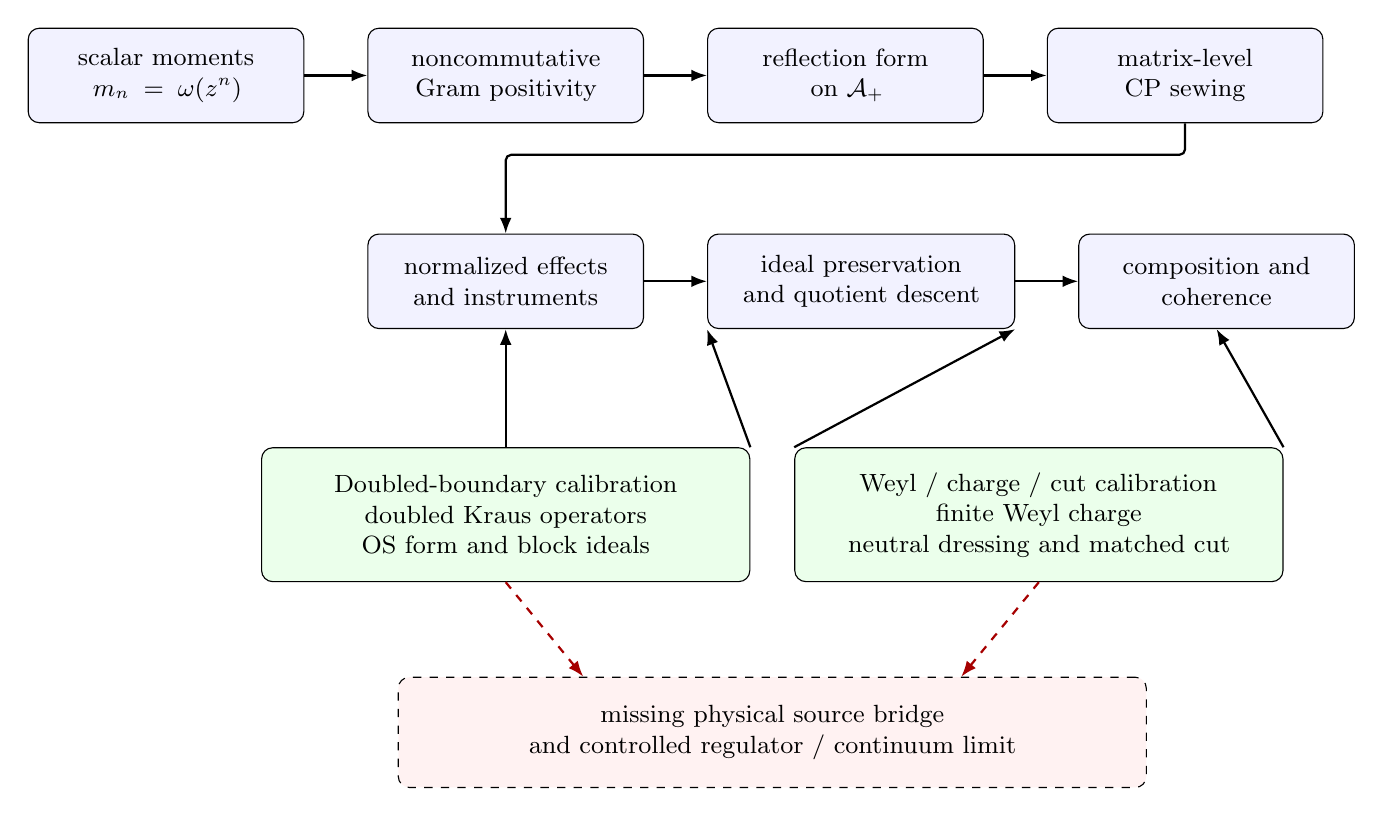
\begin{tikzpicture}[
  node distance=14mm and 8mm,
  box/.style={draw,rounded corners,align=center,font=\small,
    minimum height=12mm,text width=31mm,inner xsep=2mm,inner ysep=2mm,fill=blue!5},
  model/.style={draw,rounded corners,align=center,font=\small,
    minimum height=17mm,text width=58mm,inner sep=2mm,fill=green!8},
  open/.style={draw,dashed,rounded corners,align=center,font=\small,
    minimum height=14mm,text width=90mm,inner sep=2.5mm,fill=red!5},
  arr/.style={-{Latex[length=2mm]},thick},
  darr/.style={-{Latex[length=2mm]},thick,dashed,red!65!black}
]
\node[box] (mom) {scalar moments\\$m_n=\omega(z^n)$};
\node[box,right=of mom] (gram) {noncommutative\\Gram positivity};
\node[box,right=of gram] (os) {reflection form\\on $\A_+$};
\node[box,right=of os] (cp) {matrix-level\\CP sewing};
\node[box,below=of gram] (inst) {normalized effects\\and instruments};
\node[box,text width=35mm,right=of inst] (quot) {ideal preservation\\and quotient descent};
\node[box,right=of quot] (coh) {composition and\\coherence};
\draw[arr] (mom)--(gram);
\draw[arr] (gram)--(os);
\draw[arr] (os)--(cp);
\coordinate (returnrail) at ($(cp.south)+(0,-4mm)$);
\draw[arr,rounded corners=2pt] (cp.south)--(returnrail)-|(inst.north);
\draw[arr] (inst.east)--(quot.west);
\draw[arr] (quot.east)--(coh.west);
\node[model,below=15mm of inst] (route) {Doubled-boundary calibration\\doubled Kraus operators\\OS form and block ideals};
\coordinate (modelright) at ($(quot.south)!0.5!(coh.south)$);
\node[model,anchor=north] (ads) at (modelright |- route.north)
  {Weyl / charge / cut calibration\\finite Weyl charge\\neutral dressing and matched cut};
\coordinate (modelbase) at ($(route.south)!0.5!(ads.south)$);
\node[open,below=12mm of modelbase] (phys)
  {missing physical source bridge\\and controlled regulator / continuum limit};
\draw[arr] (route.north)--(inst.south);
\draw[arr] (route.north east)--(quot.south west);
\draw[arr] (ads.north west)--(quot.south east);
\draw[arr] (ads.north east)--(coh.south);
\draw[darr] (route.south)--([xshift=-24mm]phys.north);
\draw[darr] (ads.south)--([xshift=24mm]phys.north);
\end{tikzpicture}
}
\caption{Graphical abstract.  The horizontal and vertical boxes are distinct
acceptance gates, not implications supplied by scalar positivity.  The two exact
finite models pass selected gates.  Their dashed arrows end at an open source and
continuum bridge.}
\label{fig:graphical-abstract}
\end{figure}

\section{Introduction}

The gluing of quantum regions is often first described at the level of amplitudes.
When the objects being glued carry gauge constraints, edge sectors, mixed states, or
noncommuting observables, this scalar description is too weak.  A nonnegative number
for each closed region does not determine whether arbitrary operator insertions form a
positive Gram matrix.  A positive state on one boundary algebra does not determine
whether a geometric reflection gives a positive reconstruction form.  Even a positive
map between two algebras can fail after tensoring with an untouched ancilla, which is
precisely the stability demanded of a local physical operation.  These distinctions
are routine in operator theory and quantum information, but they are easy to blur when
``positivity of sewing'' is used as a single phrase.

The appropriate map variance is fixed throughout this paper.  A cut
$g:G\rightarrow C$ from a glued region to a cut presentation has a Heisenberg
observable pullback
\begin{equation}
  E_g:\A_C\longrightarrow\A_G,
  \qquad
  \Phi_g(\omega_G)=\omega_G\circ E_g .
  \label{eq:variance}
\end{equation}
Thus observables run from cut to glued, while states run from glued to cut.  This
separation prevents a recurrent typing error: the state dual, a reverse inclusion, and
a conditioned recovery rule are generally three different maps.

Complete positivity (CP) is the natural matrix-stable requirement on $E_g$.
Stinespring's representation theorem and the Choi--Jamio\l kowski criterion provide
the basic structural and finite-dimensional tests
\cite{Stinespring1955,Jamiolkowski1972,Choi1975}.  Normalized collections of CP outcome
maps are quantum instruments in the operational sense initiated by Davies and Lewis
\cite{DaviesLewis1970,Kraus1983}.  Reflection positivity is a separate reconstruction
condition, historically associated with the Osterwalder--Schrader axioms
\cite{OsterwalderSchrader1973,OsterwalderSchrader1975}.  General-boundary and positive
formalisms already place amplitudes, probabilities, and composition on arbitrary
boundaries \cite{Oeckl2008,Oeckl2013}.  The aim here is not to rename these established
ingredients.  It is to state exactly how they must coexist on a common quotient and to
give finite models in which their compatibility can be checked without interpretive
shortcuts.

This need is especially sharp in gravity.  Gauge-invariant gravitational observables
are dressed and generally do not form naive commuting local subsystem algebras
\cite{DonnellyGiddings2016}.  Holographic quantum error correction provides useful
finite and code-subspace analogies
\cite{AlmheiriDongHarlow2015,PastawskiEtAl2015,Harlow2017}, but an arbitrary qudit code
is not thereby a bulk gravitational theory.  In three dimensions, Virasoro TQFT and
the Ponsot--Teschner fusion data provide concrete source structures
\cite{PonsotTeschner1999,CollierEberhardtZhang2023,CollierEberhardtZhang2024}; a
hand-chosen finite Kraus family is not a compression of those structures until a
quantitative comparison is supplied.

The paper combines a typed boundary constitution with three bounded finite contributions.  First, it defines a hierarchy of scalar,
noncommutative, reflection, operational, quotient, and coherence tests with fixed map
variance.  Second, it gives exact $2\times2$ counterexamples showing that the main
upgrades are logically independent.  These examples are pedagogical and no priority
claim is made for their elementary ingredients.  Third, it presents two exact finite
calibration families.  One uses doubled Kraus operators and a canonical swap
reflection; the other uses finite Weyl charge blocks, neutral anchor dressing, and a
matched-sector quotient.  The constructions are useful because invalid controls fail
for explicit reasons and because every physical nonclaim can be localized to a missing
map or limit.

The status vocabulary is deliberately conservative.  A result marked
$\status{Std}$ is a standard theorem or consequence.  A result marked
$\status{Derived}$ is proved here from printed finite hypotheses.  A value marked
$\status{Computed}$ is reproduced by a deterministic script at the stated parameters.
An item marked $\status{Conditional}$ depends on a hypothesis not established for the
named source theory, and $\status{Open}$ denotes a missing construction.  This
taxonomy matters because the algebraic consistency of a surrogate and its physical
origin are different scientific questions.

\section{The typed positive boundary system}

Let $\Bdy$ be a category whose objects are admissible oriented boundaries and
whose morphisms are admissible regions or cobordisms.  Let $\Reg$ be a category
or directed system of regulators.

\begin{definition}[Positive boundary system]
A positive boundary system is a tuple
\begin{equation}
  \mathfrak Q=(\Bdy,\Reg,\A,\omega,\Theta,\mathcal S,
  \mathcal C,\mathcal D,\mathcal L)
  \label{eq:system}
\end{equation}
with the following typed components.
\begin{enumerate}[label=(\roman*)]
 \item $\A$ assigns a unital $*$-algebra $\A(\Sigma)$ to each boundary
 $\Sigma$, together with local subalgebras when a net is claimed.
 \item $\omega$ is a compatible family of normalized positive linear
 functionals on declared test algebras.
 \item $\Theta$ is orientation reversal or Euclidean reflection, with a
 specified positive-half algebra when OS reconstruction is claimed.
 \item $\mathcal S$ is a family of gluing correspondences or maps with declared
 domain, codomain, and direction.
 \item $\mathcal C$ is constraint data: BRST/BFV differentials, Dirac
 constraints, averaging maps, or physical ideals.
 \item $\mathcal D$ is dynamics or Ward data acting on the same physical
 structure.
 \item $\mathcal L$ is a regulator and limit package, including comparison maps
 and the topology in which convergence is asserted.
\end{enumerate}
\end{definition}

The tuple is a type system for claims.  A gluing amplitude can exist before it
is shown to be a bounded map; a bounded positive map can exist before it is
shown to be completely positive; a CP map at each cutoff can exist before it
is shown to converge on a common completion.

Complete positivity is used only after the relevant operator systems or
C*-completions and their matrix orderings have been declared.  On a merely
algebraic unbounded $*$-domain, the phrase \emph{completely positive} requires
an explicit matrix-positive cone and continuity/domain statement.

\subsection{Boundary nets and gravitational localization}

When localization is meaningful, each boundary $\Sigma$ has a family of
regions $U\subset\Sigma$ and a net $U\mapsto\A_\Sigma(U)$.  At minimum,
isotony $U\subset V\Rightarrow\A(U)\subset\A(V)$ is required.  If a boundary causal structure is
available, locality takes the form
\begin{equation}
   [\A_\Sigma(U),\A_\Sigma(V)]=0
   \quad\text{for spacelike separated }U,V.
   \label{eq:locality}
\end{equation}
Gravity complicates \eqref{eq:locality}: gauge-invariant observables may
require dressing to an asymptotic or relational anchor and may carry edge
data.  Thus the local net is a physical claim, not decorative notation.

\subsection{States and word Gram matrices}

For a unital C*-algebra a state is a positive normalized functional.  In field
theory one often begins with a dense unbounded $*$-algebra, so domains must be
printed.  We use
\begin{equation}
   \omega_\Sigma(a^*a)\ge 0,\qquad \omega_\Sigma(1)=1,
   \quad a\in\A_\Sigma^0 ,
   \label{eq:state-positive}
\end{equation}
where $\A_\Sigma^0$ is a common test algebra.  For words
$a_1,\ldots,a_n$, positivity is equivalent to
\begin{equation}
  G^\omega_{ij}=\omega(a_i^*a_j)\succeq0 .
  \label{eq:nc-gram}
\end{equation}
This is the noncommutative analogue of Hankel positivity and contains ordered
information absent from a commuting moment family.

\section{GNS reconstruction and its exact scope}

\begin{theorem}[Algebraic GNS reconstruction]
Let $\A^0$ be a unital $*$-algebra and let $\omega$ satisfy
\eqref{eq:state-positive}.  Define
\begin{equation}
   \Nw=\{a\in\A^0:\omega(a^*a)=0\}.
   \label{eq:gns-null}
\end{equation}
Then $\Nw$ is a left ideal, $\A^0/\Nw$ is a pre-Hilbert space with
\begin{equation}
   \langle[a],[b]\rangle_\omega=\omega(a^*b),
   \label{eq:gns-ip}
\end{equation}
and left multiplication gives a cyclic algebraic $*$-representation by
generally unbounded operators on the common invariant domain
$\A^0/\Nw$.  No boundedness or closability is asserted.
\end{theorem}

\begin{proof}
Cauchy--Schwarz follows by applying positivity to
$\omega((a+\lambda b)^*(a+\lambda b))$ and optimizing over $\lambda\in\C$.
If $a\in\Nw$, Cauchy--Schwarz gives $\omega(a^*b)=0$ for every $b$.
Taking $b=x^*xa$ yields
$\omega((xa)^*(xa))=\omega(a^*x^*xa)=0$, so $xa\in\Nw$.
This proves the left-ideal property and makes \eqref{eq:gns-ip} and left
multiplication well defined.  The resulting algebraic representation has
cyclic vector $[1]$
\cite{GNS1943,Segal1947}.
\end{proof}

\begin{remark}[Left-ideal warning]
The GNS null space is generally a left ideal, not a two-sided $*$-ideal.
Therefore $\A^0/\Nw$ is naturally a representation space, not automatically a
quotient algebra.  A physical observable algebra $\A/\Nw$ requires extra
two-sided and involutive stability.
\end{remark}

\begin{nonclaim}
GNS reconstruction proves neither locality, reflection positivity, Lorentzian
unitarity, covariance, closability of the represented operators, a
semiclassical metric, nor uniqueness of completion.  It constructs the minimal
cyclic algebraic representation of the supplied functional.
\end{nonclaim}

\section{Physical reduction and quotient descent}

Let $\A_{\mathrm{test}}$ be the algebra before reduction.  Three different
kernels can appear: the GNS null left ideal $\Nw$; a constraint complex, such
as a BRST differential $s$ with $s^2=0$; and a two-sided $*$-ideal $\Iphys$
through which states and operations factor.  The kernel of restriction to a
small observer algebra is a fourth, epistemic object.

\begin{definition}[Admissible physical reduction]
An admissible physical reduction is a specified construction
\begin{equation}
   (\A_{\mathrm{test}},\omega,\Theta,\mathcal S,\mathcal D)
   \longrightarrow
   (\A_{\mathrm{phys}},\omega_{\mathrm{phys}},
     \Theta_{\mathrm{phys}},\mathcal S_{\mathrm{phys}},
     \mathcal D_{\mathrm{phys}})
   \label{eq:physical-reduction}
\end{equation}
such that every object on the right is well defined and the state remains
positive.  The branch may be BRST cohomology, Dirac reduction, positive
averaging, a two-sided null quotient, or a declared composition.
\end{definition}

These branches are not interchangeable.  In a cohomological branch the state
must annihilate exact representatives and induce a positive functional on the
chosen cohomology; that construction need not be a C*-ideal quotient.  The two
quotient propositions below apply only to the stated closed-ideal branch.

\begin{proposition}[Positive state descent]
Let $\A$ be a unital C*-algebra, $I\triangleleft\A$ a closed two-sided
$*$-ideal, and $q:\A\to\A/I$ the quotient map.  A state $\omega$ factors as
$\omega=\bar\omega\circ q$ if and only if $\omega(I)=0$.  The factor
$\bar\omega$ is a state.
\end{proposition}

\begin{proof}
Factorization of a linear functional through a quotient is equivalent to
annihilating the kernel.  If $x\in(\A/I)_+$, the C*-quotient has a positive
lift $a\in\A_+$ with $q(a)=x$.  Then
$\bar\omega(x)=\omega(a)\ge0$, independently of the lift.  Normalization is
inherited.
\end{proof}

\begin{proposition}[CP quotient descent]
Let $I\triangleleft\A$ and $J\triangleleft\mathcal B$ be closed two-sided
$*$-ideals of unital C*-algebras.  Let $\Phi:\A\to\mathcal B$ be completely
positive and suppose $\Phi(I)\subset J$.  Then there is a unique completely
positive map
\begin{equation}
   \bar\Phi:\A/I\longrightarrow\mathcal B/J,\qquad
   \bar\Phi(q_A(a))=q_B(\Phi(a)).
   \label{eq:cp-descent}
\end{equation}
\end{proposition}

\begin{proof}
The ideal condition makes \eqref{eq:cp-descent} well defined.  At every matrix
level, a positive element of the quotient has a positive lift.  Complete
positivity of $\Phi$, followed by the positive quotient map $q_B$, therefore
gives positivity of every amplification of $\bar\Phi$.
\end{proof}

These are standard operator-algebra statements.  Their role is diagnostic: a
sewing map that fails ideal preservation does not act on the claimed physical
quotient.


\section{The physical completion space}

\begin{definition}[Physically admissible completion space]
Fix a sector and all declared data in \eqref{eq:system}.  The physical
completion space $\Kphys$ is the set of normalized positive states on one
fixed algebra $\A_{\mathrm{phys}}$ that satisfy:
\begin{enumerate}[label=(\roman*)]
 \item the chosen physical reduction and its domain conditions;
 \item reflection positivity when Euclidean reconstruction is claimed;
 \item matrix-level CP sewing and its composition laws;
 \item the declared dynamics or Ward identities;
 \item regulator compatibility and the claimed limiting topology;
 \item any semiclassical and infrared conditions included in the sector.
\end{enumerate}
\end{definition}

GNS or other representation data may be attached to an element of $\Kphys$,
but only together with its distinguished state.  Bare representation classes
are not elements of $\Kphys$, because restriction to an observer subalgebra is
then not defined.

Depending on the problem, $\Kphys$ may be empty, a point, a compact convex set,
or a moduli space.  Compactness is not assumed universally.  When
$\A_{\mathrm{phys}}$ is a unital C*-algebra and the gates define weak-* closed
conditions, the state space is weak-* compact and $\Kphys$ is compact as a
closed subset.  Domain conditions for unbounded algebras can spoil this simple
argument.

\begin{remark}[Emptiness is information]
If no state satisfies all gates, the candidate sector is falsified as typed.
One should not repair emptiness by silently changing the algebra, reflection,
or regulator.  Such a change defines a new candidate.
\end{remark}

\section{Restriction fibres and relational completeness}

Let $R\subset\A_{\mathrm{phys}}$ be a unital observer or relational
subalgebra.  Restriction defines
\begin{equation}
\res_R:\Kphys\longrightarrow\St(R),\qquad\rho\longmapsto\rho|_R.
\label{eq:restriction-intro}
\end{equation}

\begin{definition}[Indeterminacy relative to $R$]
The sector has gravitational indeterminacy relative to $R$ if
$\res_R$ is noninjective: there exist $\rho_1\ne\rho_2$ in $\Kphys$ such that
\begin{equation}
   \rho_1|_R=\rho_2|_R .
   \label{eq:gip}
\end{equation}
\end{definition}

\begin{definition}[Relational completeness]
The algebra $R$ is relationally complete for $\Kphys$ if $\res_R$ is
injective.  A family $\{R_i\}_{i\in I}$ is jointly complete if
\begin{equation}
  \rho\longmapsto(\rho|_{R_i})_{i\in I}
  \label{eq:joint-complete}
\end{equation}
is injective on $\Kphys$.
\end{definition}

\begin{proposition}[Observable witness]
The restriction map $\res_R$ is noninjective if and only if there are
$\rho_1,\rho_2\in\Kphys$ agreeing on $R$ and a
self-adjoint $a\in\A_{\mathrm{phys}}$ such that
$\rho_1(a)\ne\rho_2(a)$.
\end{proposition}

\begin{proof}
If restriction is noninjective, choose distinct states in the same fibre.
Distinct linear functionals differ on at least one element of the full algebra.
Writing that element as the sum of its self-adjoint real part and $i$ times
its self-adjoint imaginary part shows that the states differ on at least one
self-adjoint element.  The converse is immediate.
\end{proof}

The proposition is elementary; it is not the physical theorem.  A gravitational
realization must establish that $R$ represents a physically motivated
measurement class, both states pass every gate defining $\Kphys$, the witness
survives constraints and regulator limits, and the difference is not a gauge
relabelling.

\subsection{Relation to relational observables}

Relational observables in canonical gravity use dynamical degrees of freedom as
clocks or rods \cite{Rovelli1991,Dittrich2006}.  The restriction formulation
does not solve their construction.  It assumes that a physical relational
subalgebra has been identified and asks whether it separates admissible states.
Clock choice is therefore part of the observer specification, not a free index
on a scalar partition function.

\subsection{Epistemic and physical fibres}

Suppose a fixed-clock commutative moment problem is indeterminate.  There may
be many positive measures reproducing the same moments.  Three outcomes are
possible:
\begin{enumerate}[label=(\roman*)]
 \item additional noncommuting observables separate all measures, so the
 ambiguity was epistemic;
 \item physical constraints remove all but one completion;
 \item several completions remain in $\Kphys$ and differ on a physical
 observable, giving GIP relative to the restricted algebra.
\end{enumerate}
Only the third outcome supports a physical completion landscape.


\section{Scalar positivity and the amplified sewing test}
The following distinction prevents a scalar diagnostic from being mistaken for
complete positivity. It uses standard operator-algebra mathematics and is stated
explicitly because it changes what a finite acceptance test must measure.
\begin{proposition}[Scalar Gram consequence of positivity]
Let $\Phi:A\to B$ be positive between unital C*-algebras and let $\rho$ be a positive
functional on $B$. Then every scalar matrix $[\rho(\Phi(a_i^*a_j))]$ is positive.
\end{proposition}
\begin{proof}
For $x=\sum_jc_ja_j$ its quadratic form is $\rho(\Phi(x^*x))\geq0$.
Complete positivity is not needed.
\end{proof}
Even quantifying over every word family and every scalar target state cannot
certify CP. Transposition $T:M_2\to M_2$ is positive and passes all those tests,
while its Choi matrix is the flip, with eigenvalues $-1,1,1,1$.
The omitted direction is an entangled ancillary test, not another scalar word.
\begin{proposition}[Operator-valued Gram characterization]
A linear map $\Phi:A\to B$ is CP if and only if
$[\Phi(a_i^*a_j)]\geq0$ in $M_n(B)$ for every finite family $a_1,\ldots,a_n\in A$.
\end{proposition}
\begin{proof}
Necessity follows by amplifying a positive Gram matrix. Conversely take an
arbitrary $X\geq0$ in $M_n(A)$ and factor $X=Y^*Y$. Then
$X_{ij}=\sum_kY_{ki}^*Y_{kj}$. Each row of $Y$ gives a tested positive
operator-valued Gram, so their sum $[\Phi(X_{ij})]$ is positive. This is positivity
of every amplification.
\end{proof}
The finite constructions below establish CP through Kraus or isometry formulas;
their scalar OS and state Grams are additional tests, not substitutes for this one.

\section{Typed positivity and sewing gates}
\label{sec:gates}

\subsection{Scalar moments and noncommutative Gram matrices}

Let $\A$ be a unital $*$-algebra.  A normalized functional $\omega:\A\to\C$ is
positive when $\omega(a^*a)\geq0$ for every $a\in\A$ and $\omega(1)=1$.  If $z=z^*$
is one distinguished observable, its scalar moment sequence is
\begin{equation}
  m_n=\omega(z^n),\qquad n\geq0.
\end{equation}
Hankel positivity tests the restriction of $\omega$ to the commutative algebra
generated by $z$.  For a polynomial $p(x)=\sum_i c_i x^i$,
\begin{equation}
  \sum_{i,j}\overline c_i c_j m_{i+j}
  =\omega\bigl(p(z)^*p(z)\bigr)\geq0.
  \label{eq:hankel}
\end{equation}
This test contains no information about an operator not generated by $z$.

The noncommutative state test asks instead that every finite word family
$a_1,\ldots,a_n\in\A$ have a positive Gram matrix
\begin{equation}
  G^{\rm nc}_{ij}=\omega(a_i^*a_j)\succeq0.
  \label{eq:ncgram}
\end{equation}
For a linear functional this is equivalent to positivity, because
\begin{equation*}
c^*G^{\rm nc}c=\omega\!\left(
  \left(\sum_i c_i a_i\right)^*\left(\sum_jc_j a_j\right)\right).
\end{equation*}
The content is not the
algebraic identity but the size of the tested algebra.  A scalar moment tower is a
shadow of the noncommutative condition, not a substitute for it.

\subsection{Reflection form}

Fix an anti-linear, multiplicative, star-preserving involution
\begin{equation}
  \Theta(\lambda a)=\overline\lambda\Theta(a),\quad
  \Theta(ab)=\Theta(a)\Theta(b),\quad
  \Theta(a^*)=\Theta(a)^*,\quad \Theta^2=\id.
  \label{eq:theta-type}
\end{equation}
Let $\A_+\subseteq\A$ be a declared half-algebra or half-domain.  The reflection form
is
\begin{equation}
  \langle a,b\rangle_{\rm OS}=\omega\bigl(\Theta(a)b\bigr),
  \qquad a,b\in\A_+.
  \label{eq:osform}
\end{equation}
Reflection positivity means that every finite matrix
$[\omega(\Theta(a_i)a_j)]$ is positive semidefinite.  It depends simultaneously on
$\omega$, $\Theta$, and $\A_+$.  Positivity of $\omega(a^*a)$ does not identify
$\Theta(a)$ with $a^*$, so it does not imply \eqref{eq:osform}.  Conversely, a
reflection-positive form on a small half-algebra says nothing by itself about a process
map.

\subsection{Complete positivity, Choi matrices, and effects}

For unital $C^*$-algebras $\A_C$ and $\A_G$, a linear map
$E:\A_C\rightarrow\A_G$ is completely positive if
\begin{equation}
  E_n=\id_{\M_n}\otimes E:
  \M_n(\A_C)^+\longrightarrow\M_n(\A_G)^+
  \label{eq:cpdef}
\end{equation}
for every $n$.  In finite dimensions, $E:\M_m\to\M_n$ is CP exactly when its Choi
matrix
\begin{equation}
  C_E=\sum_{i,j=1}^{m} e_{ij}\otimes E(e_{ij})
  \label{eq:choi}
\end{equation}
is positive semidefinite.  The convention \eqref{eq:choi} fixes which tensor factor
carries the input matrix units; transposed conventions have the same spectrum but
should not be mixed inside a numerical checker.

If $K_\alpha:\Hh_G\to\Hh_C$ are finite Kraus operators, then
\begin{equation}
  E(a)=\sum_\alpha K_\alpha^*aK_\alpha
  \label{eq:kraus}
\end{equation}
is CP.  It is unital precisely when
$\sum_\alpha K_\alpha^*K_\alpha=1_G$ and subunital when the sum is at most $1_G$.
For an outcome $x$, the effect is
\begin{equation}
  e_x=E_x(1_C),\qquad 0\leq e_x\leq1_G.
\end{equation}
A finite instrument is a family $\{E_x\}_x$ of CP outcome maps satisfying
$\sum_x e_x=1_G$.  For a glued state $\omega_G$, it yields
\begin{equation}
 p(x\mid\omega_G)=\omega_G(e_x),\qquad
 \omega_{C\mid x}(a)=\frac{\omega_G(E_x(a))}{p(x\mid\omega_G)}
 \label{eq:posterior}
\end{equation}
when $p(x\mid\omega_G)>0$.  Complete positivity, subunitality, and total normalization
are three separate checks.

\begin{proposition}[Finite Stinespring compression, $\status{Std}$]
Let $V:\Hh_G\to\Hh_C\otimes\Hh_E$ be linear and let
$\pi(a)=a\otimes1_E$.  Then $E(a)=V^*\pi(a)V$ is CP.  It is unital if and only if
$V^*V=1_G$.
\end{proposition}

\begin{proof}
For $[a_{ij}]\succeq0$ and vectors $\xi_i\in\Hh_G$,
\[
 \sum_{i,j}\langle\xi_i,E(a_{ij})\xi_j\rangle
 =\sum_{i,j}\langle V\xi_i,\pi(a_{ij})V\xi_j\rangle\geq0.
\]
The unit identity is $E(1)=V^*V$.
\end{proof}

\subsection{Quotient descent and composition}

Let $N_C\triangleleft\A_C$ and $N_G\triangleleft\A_G$ be closed two-sided star
ideals.  The formula
\begin{equation}
  \overline E([a])=[E(a)]
  \label{eq:quotient-map}
\end{equation}
is representative independent exactly when
\begin{equation}
  E(N_C)\subseteq N_G.
  \label{eq:ideal-preservation}
\end{equation}
When $E$ is CP and \eqref{eq:ideal-preservation} holds, the induced map between
$C^*$-quotients is CP.  This statement applies to two-sided algebra ideals.  A GNS left
null space or a BRST cohomological quotient requires its own typing and cannot silently
be inserted into \eqref{eq:quotient-map}.

For cuts $g:G\to C$ and $h:C\to D$, the Heisenberg order is
\begin{equation}
  E_{h\circ g}=E_g\circ E_h:\A_D\longrightarrow\A_G.
  \label{eq:composition-order}
\end{equation}
Compositions and tensor products of CP maps are CP.  Outcome refinements compose by
$E_{(q,s)}=E_{g,q}\circ E_{h,s}$, and coarse graining is summation.  Coherence therefore
has an exact finite meaning once a compatible family of objects and maps is actually
declared.  A single cut does not define an entire bordism category.

\begin{table}[t]
\centering
\small
\caption{The typed gate hierarchy.  The final column is deliberately not discharged by
the finite algebraic test.}
\label{tab:gates}
\begin{tabularx}{\textwidth}{@{}p{0.19\textwidth}p{0.27\textwidth}p{0.25\textwidth}X@{}}
\toprule
Gate & Datum & Finite test & Additional physical obligation\\
\midrule
Scalar moment & $m_n=\omega(z^n)$ & Hankel/localizing matrices & identify a physical observable and its domain\\
Noncommutative state & $\omega(a_i^*a_j)$ & mixed Gram matrices & source the boundary algebra and state\\
Reflection & $(\Theta,\A_+)$ & OS Gram matrix & justify geometric reflection and half-domain\\
Sewing & $E_g:\A_C\to\A_G$ & Choi or Kraus test & derive $E_g$ from a gravitational source\\
Instrument & $\{E_{g,x}\}$ & effects sum to the unit & identify operational outcomes and records\\
Physical quotient & $(N_C,N_G)$ & $E_g(N_C)\subset N_G$ & prove nullness or constraint meaning\\
Coherence & compatible cut family & typed composition/tensor laws & control mapping-class, causal, and regulator limits\\
\bottomrule
\end{tabularx}
\end{table}

\section{Exact finite separations between the gates}
\label{sec:counterexamples}

This section records exact counterexamples in the smallest convenient algebras.  Their
purpose is not novelty but error control: every omitted gate has a concrete failure
mode.  Together they prove that the arrows in \cref{fig:graphical-abstract} are a work
program rather than a chain of automatic implications.

\begin{theorem}[Scalar moment positivity does not imply noncommutative positivity]
There is a normalized Hermitian functional on $\M_2(\C)$ whose restriction to a
projection has a positive determinate moment sequence, while the functional is not
positive on $\M_2(\C)$.
\end{theorem}

\begin{proof}
Let $z=e_{22}$ and define $\varphi(a)=\Tr(Ra)$ with
\begin{equation}
 R=\begin{pmatrix}\tfrac12&1\\[2pt]1&\tfrac12\end{pmatrix}.
 \label{eq:bad-density}
\end{equation}
Then $\varphi(1)=1$ and the restriction to $C^*(z)$ is
\[
 \varphi(f(z))=\tfrac12 f(0)+\tfrac12 f(1).
\]
Consequently $m_0=1$ and $m_n=1/2$ for $n\geq1$, and every polynomial square has
$\varphi(p(z)^*p(z))=(|p(0)|^2+|p(1)|^2)/2\geq0$.  The representing measure is the
two-atom measure $(\delta_0+\delta_1)/2$.  It is unique: any positive representing
measure obeys
$\int(x^2-x)^2\,d\mu=m_4-2m_3+m_2=0$, hence is supported on $\{0,1\}$, and $m_1$
fixes the two weights.  However, $R$ has eigenvalues $3/2$ and
$-1/2$.  For the rank-one projector
$p_-=\frac12\bigl(\begin{smallmatrix}1&-1\\-1&1\end{smallmatrix}\bigr)$,
$\varphi(p_-^*p_-)=\varphi(p_-)=-1/2$.  The singleton noncommutative Gram matrix is
therefore negative.
\end{proof}

\begin{theorem}[A positive state need not be reflection positive]
There is a faithful state $\tau$ on $\M_2(\C)$ and an anti-linear multiplicative
star-preserving involution $\Theta$ for which the OS form is negative on the full
declared half-algebra.
\end{theorem}

\begin{proof}
Take $\tau(a)=\Tr(a)/2$, $\Theta(a)=\overline a$, and declare
$\A_+=\M_2(\C)$.  Entrywise conjugation has all properties in
\eqref{eq:theta-type}.  For
\[
 j=\begin{pmatrix}0&1\\-1&0\end{pmatrix}
\]
one has $\Theta(j)=j$ and $j^2=-1$.  Hence
$\langle j,j\rangle_{\rm OS}=\tau(\Theta(j)j)=-1$, although $\tau$ is a faithful
positive state and all matrices $[\tau(a_i^*a_j)]$ are positive.
\end{proof}

\begin{theorem}[Reflection-compatible positivity does not imply complete positivity]
There is a unital positive map that preserves a reflection-positive half-algebra and
commutes with reflection, but whose Choi matrix has a negative eigenvalue.
\end{theorem}

\begin{proof}
Again use $\tau=\Tr/2$ and $\Theta(a)=\overline a$, but choose the diagonal
half-algebra $\A_+=\{\operatorname{diag}(z_1,z_2)\}$.  Then
$\tau(\Theta(a)a)=(|z_1|^2+|z_2|^2)/2\geq0$.  Let $T(a)=a^{\mathsf T}$.  Transposition
is unital, positive, trace preserving, maps $\A_+$ to itself, and commutes with
$\Theta$.  Its Choi matrix is the flip
\begin{equation}
 C_T=\sum_{i,j=1}^{2}e_{ij}\otimes e_{ji}.
\end{equation}
The flip has eigenvalue $+1$ on the three-dimensional symmetric subspace and $-1$ on
the antisymmetric vector $(\ket{01}-\ket{10})/\sqrt2$.  Thus $T$ is not CP.
\end{proof}

\begin{proposition}[Complete positivity does not imply reflection covariance]
Let $U=\operatorname{diag}(1,i)$ and $E(a)=U^*aU$ on $\M_2(\C)$.  Then $E$ is a
unital CP star automorphism, but it does not commute with
$\Theta(a)=\overline a$.
\end{proposition}

\begin{proof}
For $e_{12}$, $E(e_{12})=i e_{12}$.  Therefore
$\Theta E(e_{12})=-i e_{12}$ while $E\Theta(e_{12})=i e_{12}$.
\end{proof}

\begin{proposition}[Complete positivity does not imply normalization]
For $K=2\,1$ the map $E(a)=K^*aK=4a$ is CP but $E(1)=4\,1$.  More generally, a
Kraus representation proves CP independently of the effect inequality
$\sum_\alpha K_\alpha^*K_\alpha\leq1$.
\end{proposition}

\begin{proposition}[A unital CP map need not descend through a selected ideal]
Let $\A_C=\A_G=\C\oplus\C$ and $E(a,b)=(b,b)$.  The map is a unital star
homomorphism and hence UCP.  If $N_C=N_G=0\oplus\C$, then
$E(0,b)=(b,b)\notin N_G$ for $b\neq0$.  Consequently \eqref{eq:quotient-map} is not
well defined.
\end{proposition}

\begin{figure}[H]
\centering
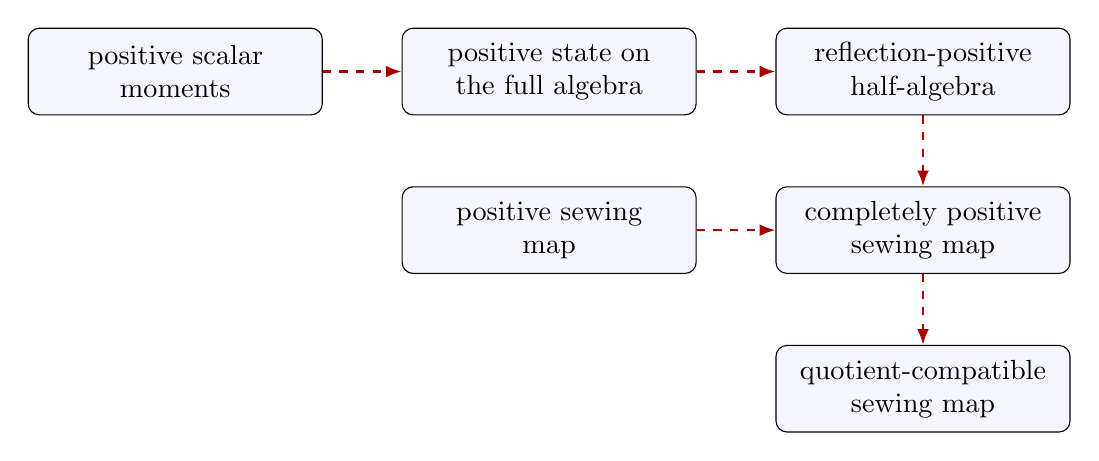
\begin{tikzpicture}[
 c/.style={draw,rounded corners,align=center,text width=35mm,minimum height=11mm,fill=blue!4},
 bad/.style={-{Latex[length=2mm]},thick,dashed,red!65!black},
 node distance=9mm and 10mm]
\node[c] (s) {positive scalar\\moments};
\node[c,right=of s] (n) {positive state on\\the full algebra};
\node[c,right=of n] (r) {reflection-positive\\half-algebra};
\node[c,below=of n] (p) {positive sewing\\map};
\node[c,right=of p] (cp) {completely positive\\sewing map};
\node[c,below=of cp] (q) {quotient-compatible\\sewing map};
\draw[bad] (s)--(n);
\draw[bad] (n)--(r);
\draw[bad] (r)--(cp);
\draw[bad] (p)--(cp);
\draw[bad] (cp)--(q);
\end{tikzpicture}
\caption{Exact nonimplications proved in this section.  Every dashed red arrow denotes
a desired upgrade that fails without an additional hypothesis.}
\label{fig:nonimplications}
\end{figure}

The separations also clarify the word ``hierarchy.''  Matrix CP is stronger than
ordinary positivity for a fixed map, but reflection positivity and quotient descent
are transverse requirements rather than simple levels of one order.  A successful
boundary process needs the intersection of these properties on compatible domains.

\section{Doubled-boundary doubled finite operational model}
\label{sec:routeT}

We now construct a finite family in which the principal gates can coexist.  The model
is abstract operator algebra: the label ``Doubled-boundary'' records its intended use as a
calibration for a future Teichm\"uller/Virasoro-TQFT compression, not an accomplished
source identification.

\subsection{Doubled channel datum}

Let $Q$ and $P$ be finite glued and cut label sets, let $h=\C^d$, and set
\begin{equation}
 K_x=\overline h\otimes h,\qquad
 \A_G=\bigoplus_{q\in Q}B(K_q),\qquad
 \A_C=\bigoplus_{p\in P}B(K_p).
 \label{eq:route-algebras}
\end{equation}
The positive half-algebras are
\begin{equation}
 \A_{G,+}=\bigoplus_q(1_{\overline h}\otimes B(h)),\qquad
 \A_{C,+}=\bigoplus_p(1_{\overline h}\otimes B(h)).
\end{equation}
Choose a finite set of triples $(p,\alpha,q)$, coefficients
$\kappa_{p\alpha\mid q}\geq0$, unitaries $F_{p\alpha\mid q}\in U(h)$, and
\begin{equation}
 s_q=\sum_{p,\alpha}\kappa_{p\alpha\mid q}\leq1.
\end{equation}
Define
\begin{equation}
 L_{p\alpha q}=\sqrt{\kappa_{p\alpha\mid q}}
       (\overline F_{p\alpha\mid q}\otimes F_{p\alpha\mid q}):K_q\to K_p
 \label{eq:doubled-kraus}
\end{equation}
and the observable pullback
\begin{equation}
 E_g(a)_q=\sum_{p,\alpha}L_{p\alpha q}^*a_pL_{p\alpha q}.
 \label{eq:route-cut}
\end{equation}
For a recorded outcome $p$, retain only the terms with that value of $p$.  Complete the
instrument by a failure algebra isomorphic blockwise to $\A_G$ and
\begin{equation}
 E_{g,\varnothing}(b)_q=(1-s_q)b_q.
 \label{eq:failure-map}
\end{equation}
The failure outcome is not cosmetic: without it a subunital cut would be silently
renormalized and the outcome probabilities would not sum to one.

In the fixed basis of $h$, let the antiunitary swap be
\begin{equation}
 J(\overline\xi\otimes\eta)=\overline\eta\otimes\xi,
 \qquad \Theta(a)=JaJ^{-1}.
 \label{eq:swap-reflection}
\end{equation}
Then $\Theta(1\otimes A)=\overline A\otimes1$ and
$\Theta(\overline F\otimes F)=\overline F\otimes F$.  The doubled form in
\eqref{eq:doubled-kraus} is selected precisely because it is fixed by the reflection.

Choose weights $w_q\geq0$ with $\sum_qw_q=1$, and define
\begin{equation}
 \Omega_d=d^{-1/2}\sum_{i=1}^{d}\overline{e_i}\otimes e_i,
 \qquad
 \omega_G(a)=\sum_qw_q\langle\Omega_d,a_q\Omega_d\rangle.
 \label{eq:fos-state}
\end{equation}
Let $Q_*=\{q:w_q>0\}$ and choose active cut labels $P_*\subseteq P$.  The inactive
whole-block ideals are
\begin{equation}
 N_G=\bigoplus_{q\notin Q_*}B(K_q),\qquad
 N_C=\bigoplus_{p\notin P_*}B(K_p).
 \label{eq:block-ideals}
\end{equation}
Assume the active-to-inactive exclusion
\begin{equation}
 \kappa_{p\alpha\mid q}=0
 \quad\text{whenever }q\in Q_*,\ p\notin P_*.
 \label{eq:active-exclusion}
\end{equation}
These are genuine two-sided $C^*$-ideals, but they model deletion of entire inactive
blocks only.  They are not generic Ward, Dirac, or BRST ideals.

\subsection{Finite operational theorem}

\begin{theorem}[Doubled finite operational sector, $\status{Derived}$]
The data \eqref{eq:route-algebras}--\eqref{eq:active-exclusion} have the following
properties.

\begin{enumerate}[label=(\roman*),leftmargin=2.1em]
\item $E_g$ and every outcome map are CP.  The completed instrument is unital, with
$E_g(1_C)_q=s_q1_{K_q}$ and
$E_{g,\varnothing}(1)_q=(1-s_q)1_{K_q}$.
\item On the center $Z_C\cong\C^P$,
\begin{equation}
 E_g(z)_q=\sum_p K(p\mid q)z_p1_{K_q},\qquad
 K(p\mid q)=\sum_\alpha\kappa_{p\alpha\mid q},
 \label{eq:center-markov}
\end{equation}
so the center evolves by a substochastic Markov kernel completed by failure mass.
\item $E_g(\A_{C,+})\subseteq\A_{G,+}$ and
$E_g\Theta_C=\Theta_GE_g$, outcome by outcome.
\item The OS form on $\A_{G,+}$ is
\begin{equation}
 \langle a,b\rangle_{\rm OS}
 =\sum_q\frac{w_q}{d}\Tr(A_q^*B_q),
 \qquad a_q=1\otimes A_q,\ b_q=1\otimes B_q.
 \label{eq:fos-os}
\end{equation}
Its radical is $N_G\cap\A_{G,+}$.
\item The represented GNS kernel is $N_G$.  Condition
\eqref{eq:active-exclusion} gives $E_g(N_C)\subseteq N_G$, hence a descended CP map
$\overline E_g:\A_C/N_C\to\A_G/N_G$.
\item If $u_x(t)$ are one-particle unitary groups satisfying
\begin{equation}
 u_p(t)F_{p\alpha\mid q}
 =e^{ic_{p\alpha q}t}F_{p\alpha\mid q}u_q(t),
 \label{eq:one-particle-intertwiner}
\end{equation}
then the doubled dynamics $W_x(t)=\overline{u_x(t)}\otimes u_x(t)$ commutes with the cut
map.
\item Successive cuts compose in the Heisenberg order
$E_{G\to D}=E_{G\to C}\circ E_{C\to D}$, and products of doubled Kraus operators are
again doubled.
\end{enumerate}
\end{theorem}

\begin{proof}
The Kraus formula gives CP at every matrix level.  Since
$L_{p\alpha q}^*L_{p\alpha q}=\kappa_{p\alpha\mid q}1$, summing the effects and adding
\eqref{eq:failure-map} proves normalization.  Central elements act as scalars in each
cut block, giving \eqref{eq:center-markov}.  For $a_p=1\otimes A_p$,
\[
 L_{p\alpha q}^*a_pL_{p\alpha q}
 =\kappa_{p\alpha\mid q}
    (1\otimes F_{p\alpha\mid q}^*A_pF_{p\alpha\mid q}),
\]
which proves half-algebra preservation.  The swap fixes every doubled Kraus block, so
reflection covariance follows term by term.

The identity
\begin{equation}
 \langle\Omega_d,(\overline A\otimes B)\Omega_d\rangle
 =\frac1d\Tr(A^*B)
 \label{eq:maxent-identity}
\end{equation}
gives \eqref{eq:fos-os}.  Strictness on every $w_q>0$ block identifies the OS radical.
On each active simple matrix block the represented GNS kernel is zero; inactive blocks
are annihilated, so the total represented kernel is $N_G$.  If $a$ is supported only on
an inactive cut block, \eqref{eq:active-exclusion} makes every active glued component of
$E_g(a)$ vanish.  This proves ideal preservation and CP descent.

Equation \eqref{eq:one-particle-intertwiner} yields
$W_p(t)L_{p\alpha q}=L_{p\alpha q}W_q(t)$ because the ordinary and conjugate phases
cancel.  Finally, if a second cut has Kraus operators $M_{r\beta p}$, substitution gives
\[
 E_1(E_2(a))=\sum_{p,\alpha,r,\beta}
 (M_{r\beta p}L_{p\alpha q})^*a_r(M_{r\beta p}L_{p\alpha q}).
\]
Operator multiplication is associative, and
$(\overline G\otimes G)(\overline F\otimes F)=\overline{GF}\otimes GF$.
\end{proof}

\begin{figure}[H]
\centering
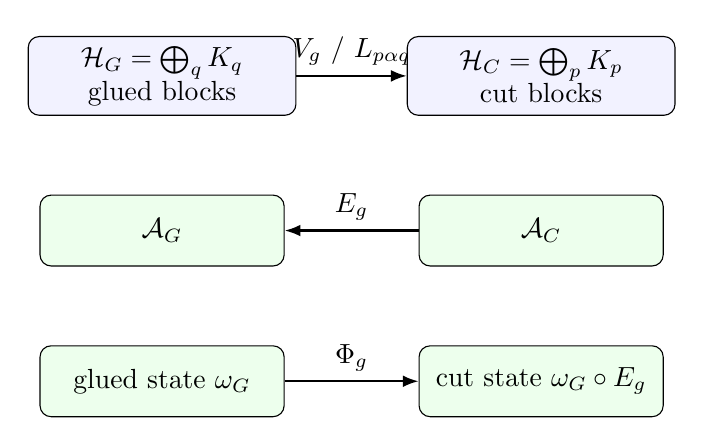
\begin{tikzpicture}[
 h/.style={draw,rounded corners,minimum width=34mm,minimum height=10mm,align=center,fill=blue!5},
 o/.style={draw,rounded corners,minimum width=31mm,minimum height=9mm,align=center,fill=green!7},
 a/.style={-{Latex[length=2mm]},thick},
 node distance=10mm and 14mm]
\node[h] (g) {$\Hh_G=\bigoplus_qK_q$\\glued blocks};
\node[h,right=of g] (c) {$\Hh_C=\bigoplus_pK_p$\\cut blocks};
\draw[a] (g)--node[above]{$V_g$ / $L_{p\alpha q}$}(c);
\node[o,below=of g] (ag) {$\A_G$};
\node[o,below=of c] (ac) {$\A_C$};
\draw[a] (ac)--node[above]{$E_g$}(ag);
\node[o,below=of ag] (sg) {glued state $\omega_G$};
\node[o,below=of ac] (sc) {cut state $\omega_G\circ E_g$};
\draw[a] (sg)--node[above]{$\Phi_g$}(sc);
\end{tikzpicture}
\caption{Variance and normalization in the Doubled-boundary finite model.  Hilbert-space
arrows point from glued to cut, observable maps point back, and state duals point
forward.  Subunital outcome effects are completed separately by the failure effect
$1-s_q$.}
\label{fig:route-variance}
\end{figure}

\subsection{Interpretive ceiling}

The theorem shows that finite matrix cones, CP cuts, reflection covariance, OS
positivity, block-ideal descent, compatible finite dynamics, and associative
composition are jointly consistent.  It does not identify $p$ or $q$ with a
principal-series momentum, $F$ with a fusion kernel, or the Markov center with a
gravitational edge observable.  The finite labels, weights, unitaries, and dynamics
were selected.  A physical three-dimensional result must instead obtain them by a
controlled compression of the positive Ponsot--Teschner/CEZ data and must prove that the
compression errors remain compatible under refinement.

\section{Two-packet instance and deterministic audit}
\label{sec:two-packet}

Take $h=\C^2$, $K=\overline h\otimes h\cong\C^4$, one glued block, and two cut blocks.
Let $X=\bigl(\begin{smallmatrix}0&1\\1&0\end{smallmatrix}\bigr)$,
$U=X\otimes X$, and
\begin{equation}
 K_0=\frac{1}{\sqrt2}1_4,\qquad
 K_1=\frac{1}{\sqrt2}U,\qquad
 E_g(a_0\oplus a_1)=\frac12(a_0+U^*a_1U).
 \label{eq:two-packet-map}
\end{equation}
The effects are both $1_4/2$, so no failure outcome is needed.  Choose
\begin{equation}
 \Omega_\lambda=\sqrt\lambda\ket{00}+\sqrt{1-\lambda}\ket{11},
 \qquad 0<\lambda<1,\quad\lambda\neq\tfrac12.
 \label{eq:lambda-state}
\end{equation}
The two outcomes have probability $1/2$.  After identifying their matrix fibers, the
posterior densities are $\rho_0=\ket{\Omega_\lambda}\bra{\Omega_\lambda}$ and
$\rho_1=U\rho_0U^*$.  Their pure-state overlap and trace distance are
\begin{equation}
 |\langle\Omega_\lambda,U\Omega_\lambda\rangle|
 =2\sqrt{\lambda(1-\lambda)},\qquad
 \frac12\norm{\rho_0-\rho_1}_1=|2\lambda-1|.
 \label{eq:posterior-distance}
\end{equation}
As states on the full direct-sum outcome algebra, however, the conditioned states have
orthogonal central support and trace distance one.  The distinction between
common-fiber distance and recorded-outcome distance is operationally important.

Let $D=\operatorname{diag}(\lambda,1-\lambda)$.  For $A,B\in\M_2(\C)$, the swap
reflection gives
\begin{equation}
 \omega_\lambda\bigl(\Theta(1\otimes A)(1\otimes B)\bigr)
 =\Tr(D^{1/2}A^*D^{1/2}B).
 \label{eq:weighted-os}
\end{equation}
In the matrix-unit basis the four OS eigenvalues are
\begin{equation}
 \lambda,\quad\sqrt{\lambda(1-\lambda)},\quad
 \sqrt{\lambda(1-\lambda)},\quad1-\lambda,
 \label{eq:os-eigenvalues}
\end{equation}
so the form is positive definite for $0<\lambda<1$.  If
$h=\operatorname{diag}(0,\Delta)$, the semigroup
$T_t(A)=e^{-th}Ae^{-th}$ is self-adjoint and contractive in this OS inner product; its
positive generator $L_h+R_h$ has spectrum
\begin{equation}
 0,\quad\Delta,\quad\Delta,\quad2\Delta.
 \label{eq:generator-spectrum}
\end{equation}
This is a finite reconstruction calibration, not physical Lorentzian time.

The companion script was rerun for $\lambda=0.7$, $\Delta=1.3$, and tolerance
$10^{-12}$.  Selected results are shown in \cref{tab:route-audit}.  The Choi minimum of
$-5.55\times10^{-17}$ is consistent with roundoff and is far above the negative
tolerance threshold.  Invalid controls deliberately detect superunital Kraus weights,
a dropped outcome, a singular OS state, and an obsolete reflection convention.

\begin{table}[t]
\centering
\caption{Rerun of the Doubled-boundary two-packet checker.  Analytic identities are the proof;
the floating-point values are regression evidence.}
\label{tab:route-audit}
\begin{tabular}{@{}lr@{}}
\toprule
Quantity & Rerun value\\
\midrule
$\norm{V^*V-1}$ & $2.22\times10^{-16}$\\
instrument normalization residual & $2.22\times10^{-16}$\\
minimum outcome Choi eigenvalue & $-5.55\times10^{-17}$\\
reflection-covariance residual (seeded sample) & $0$\\
smallest OS Gram eigenvalue & $0.3000000000000001$\\
OS spectrum-formula residual & $1.24\times10^{-16}$\\
identified-fiber posterior distance & $0.4$\\
recorded-outcome posterior distance & $1$\\
generator spectrum & $0,1.3,1.3,2.6$\\
overall & \status{Pass}\\
\bottomrule
\end{tabular}
\end{table}

The checker exhausts the declared two-outcome Choi matrices, the OS basis, posterior
formulae, and generator spectrum.  Reflection is checked on a seeded sample in addition
to the analytic proof.  It does not numerically instantiate every general ideal,
dynamics, failure-posterior, or multi-cut case in \cref{sec:routeT}.

\section{Finite Weyl charge, dressing, and matched sewing}
\label{sec:adsfinite}

The second calibration family has a different purpose.  It tests whether charge
sectors, an invariant subalgebra, a neutralizing anchor, a retained edge center, and a
matched-sector cut can coexist with CP and exact quotient descent.  Slot names are
mnemonic only.  In particular, a slot called $g_+$ or $g_-$ is not a graviton helicity,
and a slot called $\phi$ is not a continuum field.

\subsection{Charge: discrete Weyl algebra and charge physicalization}

Fix an odd prime $d$, let $\zeta=e^{2\pi i/d}$, and let $h=\C^d$.  With
$X\ket n=\ket{n+1}$ and $Z\ket n=\zeta^n\ket n$, define for
$u=(a,b)\in\Fd^2$
\begin{equation}
 W(u)=\zeta^{ab/2}X^aZ^b,\qquad
 \sigma(u,v)=ab'-ba'.
 \label{eq:weyl-def}
\end{equation}
All exponents are evaluated in $\Fd$.  Direct multiplication gives
\begin{equation}
 W(u)W(v)=\zeta^{-\sigma(u,v)/2}W(u+v),\qquad
 W(u)^*=W(-u),\qquad
 \Tr(W(u)^*W(v))=d\,\delta_{u,v}.
 \label{eq:weyl-laws}
\end{equation}
The finite Weyl relation is not the continuum CCR.  Indeed, no finite-dimensional
matrices satisfy $[Q,P]=i\hbar1$ because the traces of the two sides disagree.

For each side $r\in\{L,R\}$ take four slots
$S=\{g_+,g_-,\phi,a\}$ and
\begin{equation}
 \Hh_r^{\rm kin}=\bigotimes_{s\in S}h_{r,s},\qquad
 \A_r^{\rm kin}=B(\Hh_r^{\rm kin})\cong\M_{d^4}(\C).
\end{equation}
Define the finite charge representation
\begin{equation}
 U_r(t)=Z_{r,g_+}^tZ_{r,g_-}^tZ_{r,\phi}^tZ_{r,a}^t,\qquad t\in\Fd,
\end{equation}
and Fourier projectors
\begin{equation}
 P_{r,q}=\frac1d\sum_{t\in\Fd}\zeta^{-qt}U_r(t).
 \label{eq:charge-projectors}
\end{equation}
Character orthogonality implies
\begin{equation}
 P_{r,q}P_{r,q'}=\delta_{q,q'}P_{r,q},\qquad
 \sum_qP_{r,q}=1,\qquad \rank P_{r,q}=d^3.
 \label{eq:projector-laws}
\end{equation}
The finite-group average
\begin{equation}
 \mathcal F_r(A)=\frac1d\sum_{t\in\Fd}U_r(t)AU_r(t)^*
 \label{eq:group-average}
\end{equation}
is a UCP conditional expectation onto
\begin{equation}
 \A_r^{\rm inv}=\bigoplus_{q\in\Fd}B(P_{r,q}\Hh_r^{\rm kin}),
 \qquad
 Z_r^{\rm edge}=\Span\{P_{r,q}\}.
 \label{eq:invariant-algebra}
\end{equation}
The proof is finite: each conjugation is a UCP star automorphism, their average is UCP,
group translation proves idempotence, and the spectral decomposition identifies the
range.  For any density matrix $\rho$, the functional
$\omega^{\rm inv}(A)=\Tr(\rho\,\mathcal F_r(A))$ is positive on the entire mixed
four-slot algebra.  This mixed state cone is stronger than four separate slot tests.

\subsection{Dressing: neutral anchor dressing}

Let $u=(u_{g_+},u_{g_-},u_\phi)$ label the three internal slots, with
$u_s=(a_s,b_s)$, and put
\begin{equation}
 c_{\rm int}(u)=a_{g_+}+a_{g_-}+a_\phi\in\Fd.
\end{equation}
The neutral dressed Weyl generator is
\begin{equation}
 D_{r,0}(u)=W_r^{\rm int}(u)X_{r,a}^{-c_{\rm int}(u)}.
 \label{eq:dressing}
\end{equation}
Because anchor powers commute among themselves and act on a distinct tensor factor,
the internal Weyl multiplier is unchanged:
\begin{equation}
 D_{r,0}(u)D_{r,0}(v)
 =\zeta^{-\Sigma_{\rm int}(u,v)/2}D_{r,0}(u+v),
 \qquad D_{r,0}(u)^*=D_{r,0}(-u).
 \label{eq:dressed-weyl}
\end{equation}
Thus $W_r^{\rm int}(u)\mapsto D_{r,0}(u)$ extends to an injective unital star
homomorphism
\begin{equation}
 \iota_{r,0}:\M_{d^3}(\C)\hookrightarrow\A_r^{\rm kin}.
\end{equation}
The internal and anchor charge phases cancel, so
$\Ad U_r(t)(D_{r,0}(u))=D_{r,0}(u)$.  Consequently the dressed algebra lies in
$\A_r^{\rm inv}$ and acts faithfully in every charge block.

Changing an anchor origin by $s\in\Fd$ gives
\begin{equation}
 \iota_{r,s}=\Ad(Z_{r,a}^s)\circ\iota_{r,0},\qquad
 C_r(s_2,s_1)=Z_{r,a}^{s_2-s_1},
 \label{eq:anchor-cocycle}
\end{equation}
with the exact cocycle law
$C_r(s_3,s_2)C_r(s_2,s_1)=C_r(s_3,s_1)$.  Computational-basis conjugation satisfies
$\Theta_r(D_{r,0}(u))=D_{r,0}(\kappa u)$, where $\kappa(a,b)=(a,-b)$.  This is
reflection covariance, not OS positivity.

A useful positive control is the bounded slot quadratic
\begin{equation}
 T_{{\rm slot},r}=(1-Y_r)^*(1-Y_r)+(1-Z_r^{\rm dress})^*(1-Z_r^{\rm dress}),
 \label{eq:tslot}
\end{equation}
where $Y_r=X_{r,\phi}X_{r,a}^{-1}$ and $Z_r^{\rm dress}=Z_{r,\phi}$.  It is positive,
charge invariant, and anchor covariant.  It has no spacetime index, conservation law,
or Ward identity and is not a stress tensor.

\subsection{Cut: matched-charge cut and quotient}

Define the cut and glued Hilbert spaces
\begin{align}
 \Hh_C&=\bigoplus_{q_L,q_R\in\Fd}
   \Hh_L(q_L)\otimes\Hh_R(q_R),\\
 \Hh_G&=\bigoplus_{q\in\Fd}
   \Hh_L(q)\otimes\Hh_R(-q),
 \label{eq:matched-spaces}
\end{align}
and let $\A_C$ and $\A_G$ be the corresponding block-diagonal direct sums of full
matrix algebras.  Let $V_g:\Hh_G\to\Hh_C$ be the canonical inclusion into the matched
subspace.  If $\Pi_q^C$ projects onto the cut block $(q,-q)$, set
\begin{equation}
 E_g(a)=V_g^*aV_g,\qquad
 E_{g,q}(a)=V_g^*\Pi_q^Ca\Pi_q^CV_g.
 \label{eq:matched-instrument}
\end{equation}

\begin{theorem}[Matched-charge finite process package, $\status{Derived}$]
The map $E_g:\A_C\to\A_G$ is UCP and the $E_{g,q}$ form a normalized CP
instrument with effects $e_q^G$.  On the cut center,
\begin{equation}
 E_g(\Pi_{q_L,q_R}^C)=\delta_{q_R,-q_L}e_{q_L}^G.
 \label{eq:center-match}
\end{equation}
The unmatched block algebra
\begin{equation}
 I_{\rm unmatch}=\bigoplus_{q_L+q_R\neq0}
 B(\Hh_L(q_L)\otimes\Hh_R(q_R))
 \label{eq:unmatched-ideal}
\end{equation}
is a two-sided star ideal, $\ker E_g=I_{\rm unmatch}$, and
$\A_C/I_{\rm unmatch}\cong\A_G$.  On the declared block algebras, $E_g$ is the
associated unital star quotient homomorphism.  It preserves the dressed Weyl relations,
edge center, slot quadratics, and computational reflection.  A compatible family of
such inclusions composes in the order \eqref{eq:composition-order} and has exact
outcome refinement and tensor-product coherence.
\end{theorem}

\begin{proof}
Compression by the isometry $V_g$ proves UCP.  Replacing $V_g$ by
$\Pi_q^CV_g$ proves CP of each outcome, and orthogonality of the matched block
projectors gives
$\sum_qE_{g,q}=E_g$ and $\sum_qE_{g,q}(1_C)=1_G$.  The inclusion has range only in
$(q,-q)$ blocks, yielding \eqref{eq:center-match}.  Because $\A_C$ is explicitly block
diagonal, restriction deletes exactly the unmatched full matrix blocks and preserves
products and stars on every matched block.  This proves the kernel and quotient
statements.  All dressed generators and center projectors are block diagonal, so their
relations survive restriction.  The inclusion is real in the computational basis,
which gives $\Theta_GE_g=E_g\Theta_C$.  Composition follows from
$(V_hV_g)^*a(V_hV_g)=V_g^*(V_h^*aV_h)V_g$; outcome and tensor statements follow by
the same calculation.
\end{proof}

For a glued state $\rho$, the outcome probabilities and normalized cut posteriors are
\begin{equation}
 p(q\mid\rho)=\rho(e_q^G),\qquad
 \Phi_{g,q}(\rho)(a)=\frac{\rho(E_{g,q}(a))}{p(q\mid\rho)}.
\end{equation}
The reverse observable inclusion
$J_g(b)=V_gbV_g^*$ is an injective nonunital star homomorphism with
$J_g(1_G)=\Pi_{\rm match}$.  A cut-to-glued conditioned state rule
\begin{equation}
 \Gamma_g(\sigma)(b)=\frac{\sigma(J_g(b))}{\sigma(\Pi_{\rm match})}
\end{equation}
is nonlinear on the full state space.  Neither $J_g$ nor $\Gamma_g$ is the state dual
$\Phi_g=\rho\circ E_g$.

\begin{figure}[H]
\centering
\resizebox{\textwidth}{!}{%
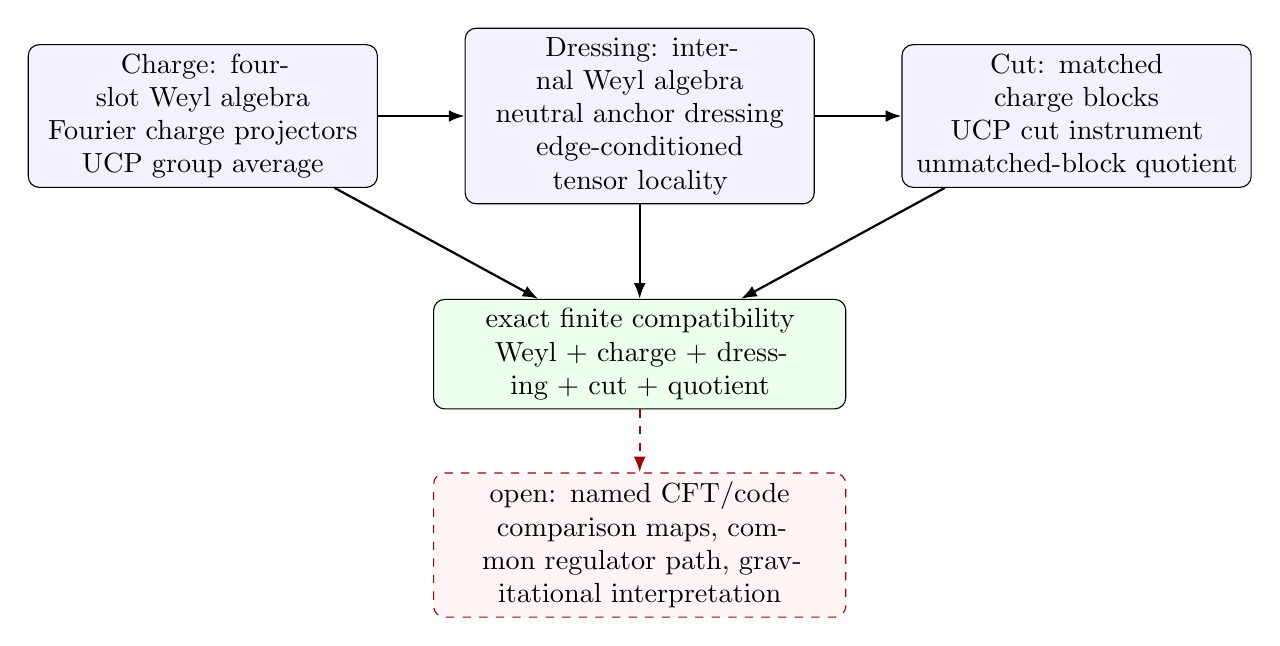
\begin{tikzpicture}[
 b/.style={draw,rounded corners,align=center,text width=42mm,minimum height=11mm,fill=blue!5},
 stage/.style={draw,rounded corners,align=center,text width=50mm,minimum height=11mm,fill=green!7},
 a/.style={-{Latex[length=2mm]},thick},
 node distance=8mm and 11mm]
\node[b] (m1) {Charge: four-slot Weyl algebra\\Fourier charge projectors\\UCP group average};
\node[b,right=of m1] (m2) {Dressing: internal Weyl algebra\\neutral anchor dressing\\edge-conditioned tensor locality};
\node[b,right=of m2] (m3) {Cut: matched charge blocks\\UCP cut instrument\\unmatched-block quotient};
\draw[a] (m1)--(m2);
\draw[a] (m2)--(m3);
\node[stage,below=12mm of m2] (exact) {exact finite compatibility\\Weyl $+$ charge $+$ dressing $+$ cut $+$ quotient};
\draw[a] (m1)--(exact);
\draw[a] (m2)--(exact);
\draw[a] (m3)--(exact);
\node[stage,draw=red!65!black,dashed,fill=red!4,below=of exact] (bridge) {open: named CFT/code comparison maps, common regulator path, gravitational interpretation};
\draw[a,dashed,red!65!black] (exact)--(bridge);
\end{tikzpicture}
}
\caption{The Weyl/charge/cut logical flow.  Exact finite compatibility terminates before the
physical bridge.}
\label{fig:m1m3}
\end{figure}
\subsection{Rerun evidence and verification ceiling}

At $d=3$, the companion checker exhausts the one-slot Weyl labels and the charge
projector identities.  It samples a group-average input, a positive averaged output,
one dressed Weyl pair, and a cut state using a fixed seed.  The rerun values in
\cref{tab:ads-audit} all satisfy the declared tolerance $2\times10^{-11}$.

\begin{table}[t]
\centering
\caption{Selected rerun values for the $d=3$ Weyl/charge/dressing/cut checker.}
\label{tab:ads-audit}
\begin{tabular}{@{}lr@{}}
\toprule
Quantity & Rerun value\\
\midrule
single-mode Weyl product residual & $2.59\times10^{-15}$\\
projector completeness residual & $1.91\times10^{-15}$\\
projector ranks & $27,27,27$\\
sample group-average idempotence residual & $5.05\times10^{-14}$\\
sample positive-output invariance residual & $1.40\times10^{-12}$\\
dressing charge-invariance residual & $6.86\times10^{-15}$\\
sample dressed-Weyl residual & $2.37\times10^{-14}$\\
anchor-change residual & $4.73\times10^{-15}$\\
$T_{\rm slot}$ minimum eigenvalue & $1.2679491924$\\
cut-space / glued-space dimensions & $6561/2187$\\
sample outcome probabilities & $0.2,0.3,0.5$\\
instrument probability residual & $1.11\times10^{-16}$\\
successive-cut charge-set difference & $0$\\
overall & \status{Pass}\\
\bottomrule
\end{tabular}
\end{table}

The checker detects three invalid controls: a naively truncated CCR, an undressed
charged operator, and an incomplete instrument.  It does not construct the full Choi
matrix of the $6561$-dimensional matched-charge map, nor is that needed for the theorem: the analytic
compression proof establishes CP at every matrix level.  The numerical run is a
regression check on selected coordinates, not a substitute for that proof.

\section{A deterministic acceptance protocol}
\label{sec:protocol}

The two models suggest a compact protocol that separates analytic obligations from
finite implementation checks.  Given finite algebras, outcome maps, reflections, and
ideals, one first fixes map variance and bases.  The Choi matrix is then constructed
from \eqref{eq:choi} or CP is proved from an explicit Stinespring/Kraus representation.
Effects are evaluated independently and summed to the identity.  Reflection is checked
as an anti-linear map, including multiplicativity and star compatibility, before its
intertwining with each outcome map is tested.  Quotient descent is verified by applying
the map to a basis of the outgoing ideal and checking membership in the incoming ideal.
Finally, sequential maps are compared in the Heisenberg order
\eqref{eq:composition-order}; outcome sums are checked before any conditioned
renormalization.

\small
\begin{longtable}{@{}p{0.15\textwidth}p{0.32\textwidth}p{0.19\textwidth}p{0.21\textwidth}@{}}
\caption{Acceptance protocol and the strength of each evidence type.}
\label{tab:protocol}\\
\toprule
Check & Exact criterion & Finite implementation & What a pass does not prove\\
\midrule
\endfirsthead
\toprule
Check & Exact criterion & Finite implementation & What a pass does not prove\\
\midrule
\endhead
CP & $C_E\succeq0$ or $E(a)=V^*\pi(a)V$ & minimum Choi eigenvalue with tolerance & physical origin of $E$\\
Effect & $0\leq E_x(1)\leq1$ & effect eigenvalues & total normalization\\
Instrument & $\sum_xE_x(1)=1$ & norm residual & interpretation of outcomes\\
Reflection type & \eqref{eq:theta-type} & basis and random-product residuals & geometric OS reflection\\
OS positivity & $[\omega(\Theta(a_i)a_j)]\succeq0$ & declared half-basis Gram spectrum & continuum reconstruction axioms\\
Ideal descent & $E(N_C)\subseteq N_G$ & ideal-basis membership & physical nullness of the ideal\\
Composition & $E_{h\circ g}=E_gE_h$ & matrix residual or Kraus multiplication & a complete cut category\\
Source bridge & comparison square and error bounds & not supplied here & continuum gravity\\
\bottomrule
\end{longtable}
\normalsize

A tolerance must be paired with a scaling convention.  A minimum Choi eigenvalue of
$-10^{-16}$ is harmless only when matrix norms are order one and the declared tolerance
is much larger.  Conversely, a sampled residual of zero does not establish an identity
on an untested space.  The correct report therefore labels tests as exhaustive,
analytic, or seeded-sample.  Both scripts used here print their scope and deliberately
failing controls; that practice guards against a checker whose pass condition is
vacuous.

\section{The missing physical source bridge}
\label{sec:bridge}

Finite consistency is a necessary but weak result.  The source bridge asks whether the
finite data arise as controlled compressions of a specified gravitational construction
and whether the compatibility gates survive a directed limit.  This is not a matter of
renaming the finite labels.

\subsection{Three-dimensional source comparison}

A Doubled-boundary promotion would begin with an actual principal-series Hilbert/form datum,
Ponsot--Teschner or Virasoro-TQFT sewing kernels, and their positive row measure
\cite{PonsotTeschner1999,CollierEberhardtZhang2023}.  For a regulator $R$, one would need
packet embeddings or compressions
\begin{equation}
 C_{X,R}:\A_X^{\rm fin}(R)\longrightarrow\A_X^{\rm src}(R)
\end{equation}
and a source cut map $E_g^{\rm src}(R)$.  The finite square has a meaningful defect only
after all maps exist:
\begin{equation}
 \varepsilon_{\rm cut}^{\rm cb}(R)
 =\norm{C_{G,R}E_g^{\rm fin}-E_g^{\rm src}(R)C_{C,R}}_{\rm cb}.
 \label{eq:cez-defect}
\end{equation}
Unital, state, center, reflection, presentation, composition, and dynamics defects must
be bounded on one common domain.  A polar correction or failure outcome may repair a
finite compression, but its correction norm must also tend to zero.  In addition, the
directed family must preserve the matrix cones and states rather than merely converge
entrywise.  No such complete comparison family is constructed here; consequently
$\varepsilon_{\rm cut}^{\rm cb}$ is presently undefined, not zero.

The distinction is substantive.  Virasoro TQFT describes a precise fixed-topology
on-shell sector and brings noncompact fusion and mapping-class structures that are
absent from a generic finite matrix channel
\cite{CollierEberhardtZhang2023,CollierEberhardtZhang2024}.  Compact packet windows must
control leakage, branch and chart conventions, discrete or vacuum contributions, and
the convergence topology of sums of CP correspondences.  The Doubled-boundary theorem provides
the target type for such a comparison but proves none of those estimates.

\subsection{Four-dimensional code comparison}

For the Weyl/charge model, a physical bridge requires a named sequence of CFT or code
algebras, not only an analogy with holographic codes.  One would need maps
\begin{equation}
 C_{C,\lambda}:\A_C^{\rm fin}\to\A_C^{\rm code}(\lambda),\qquad
 C_{G,\lambda}:\A_G^{\rm fin}\to\A_G^{\rm code}(\lambda),
 \label{eq:code-comparison}
\end{equation}
together with a physical $E_g^{\rm code}(\lambda)$.  The analogue of
\eqref{eq:cez-defect} must vanish along a declared large-$N$/cutoff path, while product,
star, state, charge, dressing, localization, reflection, instrument, posterior, and
coherence errors vanish compatibly.

Holographic codes show that finite isometries can capture important reconstruction and
entropy patterns \cite{PastawskiEtAl2015,Harlow2017}.  They do not license identifying
the present four slots with gravitons and matter.  Moreover, actual gravitational
dressing obstructs naive exact tensor-factor locality
\cite{DonnellyGiddings2016}.  The exact commutativity of the left and right finite tensor
factors is therefore a surrogate control, not evidence for locality of observables with
shared asymptotic dressing.  A physical bridge must quantify that discrepancy rather
than hide it in slot names.

\subsection{Constraint meaning and continuum limits}

In both families the quotient ideals are elementary whole-block ideals.  Their
algebraic descent is exact, but their physical meaning is selected by hand.  A
gravitational quotient would normally involve constraints, Ward identities, edge
charges, gauge cohomology, or state-dependent null spaces.  One must prove that the
relevant null structure is stable under every sewing map and reflection, and that the
quotient cone remains proper.  It is not sufficient to observe that a chosen direct-sum
block can be deleted.

Similarly, a directed limit needs compatible embeddings, uniformly controlled maps,
states, and reflections, and a declared topology.  Entrywise convergence of finite
matrices does not automatically preserve complete positivity on an unbounded dense
domain.  Even after a positive continuum process is obtained, semiclassical Einstein
dynamics and an infrared observable map remain additional obligations.  This paper
therefore stops at finite calibration by design.

\section{Discussion}

The central result is negative and constructive at once.  Negatively, scalar moments,
positive states, reflection forms, positive process maps, CP maps, normalized
instruments, and physical quotients are not interchangeable.  The elementary examples
in \cref{sec:counterexamples} expose a distinct failure at each substitution.
Constructively, the Doubled-boundary and Weyl/charge/cut families demonstrate that selected versions of
all these interfaces can coexist without contradiction in finite matrix algebra.

The doubled-boundary model is strongest where reflection and operational normalization
are concerned.  The choice $\overline F\otimes F$ simultaneously preserves the
half-algebra, fixes the maximally entangled vector, and cancels phases in both reflection
and dynamics.  The failure block turns subunital cutting into a genuine normalized
instrument.  The price is rigidity: these conveniences are engineered.  A source
kernel need not have exactly doubled unitary blocks, and a nonmaximally entangled state
requires a separate OS proof, as the two-packet example illustrates.

The Weyl/charge model is strongest where edge centers, invariant reduction, dressing,
and quotient matching are concerned.  Finite-group averaging supplies a standard UCP
conditional expectation, and neutral anchor dressing embeds a full internal matrix
algebra faithfully into every retained charge sector.  Matched-sector compression is
not merely CP but a star quotient homomorphism on the declared block-diagonal algebra.
The price is again physical distance: modulo-$d$ charge is not a gravitational Gauss
law, the anchor is not a gravitational line dressing, and $T_{\rm slot}$ is not a stress
tensor.

The literature boundary is correspondingly narrow.  Stinespring representations,
Choi matrices, Kraus operations, instruments, OS reconstruction, conditional
expectations, and operator-algebra quantum error correction are established structures
\cite{Stinespring1955,Choi1975,DaviesLewis1970,OsterwalderSchrader1973,BenyKempfKribs2007}.
The contribution of the present framework is not their invention.  It is the explicit
requirement that matrix CP, operational normalization, reflection, ideal descent, edge
records, and composition be checked on one typed family, plus exact finite reference
implementations and explicit stop lines.  Whether this synthesis has gravitational
content is decided only by the source bridges in \cref{sec:bridge}.

The finite models can still be scientifically useful before that bridge exists.  They
serve as unit tests for proposed continuum formulae.  A candidate compression that
produces a sign-indefinite Choi matrix, loses a failure outcome, deletes an active edge
block, reverses map variance, or violates reflection covariance fails immediately.
They also distinguish a genuine obstruction from numerical instability: a transpose
map has an exact Choi eigenvalue $-1$, whereas the two-packet Choi minimum of order
$10^{-17}$ is roundoff around an analytic positive matrix.

\section{Limitations and nonclaims}

The main mathematical limitation is finite dimensionality.  Matrix algebras avoid
unbounded operator domains, type-III local structure, infrared sectors, anomalies, and
the topology of regulator removal.  The quotient ideals are whole direct-sum blocks,
not cohomological or dynamical constraint ideals.  The OS forms are finite Gram forms,
not a verification of all Osterwalder--Schrader axioms.  Dynamics in the Doubled-boundary model
is a selected finite unitary or contraction semigroup, not a Hamiltonian constraint or
physical time.

The numerical evidence is intentionally subordinate to the proofs.  The Doubled-boundary
checker exhausts its small Choi and OS matrices but samples some covariance identities.
The $d=3$ Weyl checker exhausts one-slot Weyl and projector identities but samples
group-average and dressing inputs and does not build the full matched-charge Choi matrix.  Passing
results show that the implementations agree with selected analytic formulae at one
finite regulator.  They do not establish a convergence theorem.

No result here establishes a CEZ packet origin, a Moore--Seiberg coherent cut category,
a physical AdS/CFT code, a graviton, a scalar QFT, a renormalized stress tensor,
diffeomorphism constraints, anomaly cancellation, semiclassical Einstein equations,
gravitational EFT recovery, a UV completion, or an empirical prediction.  The title's
``physical quotient'' should therefore be read as a typed target instantiated by exact
finite block quotients, not as a claim that the model's ideals have already been
identified with the null ideal of quantum gravity.

\section{Conclusion}

A boundary quantum theory cannot be certified by one scalar notion of positivity.
Noncommutative state positivity, reflection positivity, matrix-completely-positive
sewing, effect normalization, quotient descent, and coherent composition answer
different questions.  Exact $2\times2$ counterexamples show that omitting any of these
questions can change the answer from positive to negative.

The two finite families constructed here pass a substantial common subset of the
resulting gate stack.  They provide exact formulas, analytic proofs, deterministic
checks, invalid controls, and a clear map variance.  This is enough to establish the
internal consistency and nontriviality of the selected operator-algebraic interfaces.
It is not enough to establish quantum gravity.  The decisive next result must construct
one physical source family and prove that its comparison maps, CP sewing, reflection,
constraints, edge records, and regulator limit close together.  Until then, the finite
models should be used as calibration standards and falsifiers, not as evidence for a
continuum gravitational sector.

\appendix

\section{Choi and instrument conventions}

For $E:\M_m\to\M_n$ our Choi convention is \eqref{eq:choi}.  If
$E(a)=K^*aK$ with $K:\C^n\to\C^m$, then vectorization gives
\begin{equation}
 C_E=\operatorname{vec}(K)\operatorname{vec}(K)^*
\end{equation}
up to the fixed vectorization order, and is therefore positive.  A Kraus sum gives a
sum of such rank-one matrices.  The eigenvalues depend neither on a simultaneous basis
change nor on which consistent Choi tensor convention is chosen.

In Heisenberg variance, $E_x(1)$ is an effect in the input/glued algebra.  If
$\omega_G$ is a state, the probability is $\omega_G(E_x(1))$.  The normalized posterior
is a state on the outcome algebra, not an operator in the glued algebra.  For a direct
sum of recorded outcomes, two conditioned states in disjoint blocks have trace distance
one even when their internal fiber states are close.  Forgetting the center is a
separate channel and should be declared before comparing fiber densities.

For successive cuts, if $K_\alpha:\Hh_G\to\Hh_C$ and
$M_\beta:\Hh_C\to\Hh_D$, then
\begin{equation}
 E_{G\to C}(E_{C\to D}(a))
 =\sum_{\alpha,\beta}(M_\beta K_\alpha)^*a(M_\beta K_\alpha).
\end{equation}
This formula fixes both the map order and the product order of Kraus operators.

\section{Expanded verification of the finite separations}

For the scalar-moment example, every Hankel quadratic is explicitly
\begin{equation}
 \sum_{i,j=0}^{N}\overline c_i c_jm_{i+j}
 =\frac12\left|\sum_{i=0}^{N}c_i0^i\right|^2
  +\frac12\left|\sum_{i=0}^{N}c_i\right|^2,
\end{equation}
with the convention $0^0=1$.  It is nonnegative at every order.  The negative
noncommutative direction $p_-$ is invisible because $p_-\notin C^*(e_{22})$.

For transposition on $\M_2$, the Choi matrix in the ordered basis
$\ket{00},\ket{01},\ket{10},\ket{11}$ is
\begin{equation}
 C_T=
 \begin{pmatrix}
 1&0&0&0\\
 0&0&1&0\\
 0&1&0&0\\
 0&0&0&1
 \end{pmatrix}.
\end{equation}
The central $2\times2$ block has eigenvalues $\pm1$.  Thus a scalar positivity test or
a test on the diagonal half-algebra cannot see the ancillary antisymmetric direction
that violates CP.

For the quotient counterexample, the quotient map
$q:\C\oplus\C\to\C$ associated with $N=0\oplus\C$ keeps the first coordinate.  If a
descended map $\overline E$ existed, it would obey
$\overline E(q(0,b))=q(E(0,b))$.  The left side is $\overline E(0)=0$, while the right
side is $q(b,b)=b$.  This contradiction proves failure of representative independence.

\section{Doubled-boundary proof details}

For the posterior formula in the maximally entangled FOS state, the doubled unitary
fixes $\Omega_d$:
\begin{equation}
 (\overline F\otimes F)\Omega_d=\Omega_d.
\end{equation}
Consequently the unnormalized outcome functional is
\begin{equation}
 \Phi_{g,p}(\omega_G)(a_p)
 =\sum_{q,\alpha}w_q\kappa_{p\alpha\mid q}
   \langle\Omega_d,a_p\Omega_d\rangle,
\end{equation}
and
\begin{equation}
 p(p\mid\omega_G)=\sum_{q,\alpha}w_q\kappa_{p\alpha\mid q},\qquad
 p(\varnothing\mid\omega_G)=\sum_qw_q(1-s_q).
\end{equation}
Their sum is one.  In the two-packet nonmaximal state, this simplification is rederived
directly rather than inherited from maximal entanglement.

The GNS null left ideal of a vector state on one simple matrix block is not itself a
two-sided ideal.  The represented kernel, however, is a two-sided ideal and is zero on
every active simple block.  This is why \cref{sec:routeT} uses the represented kernel
and whole inactive blocks for quotient descent.  Replacing $N_G$ by an arbitrary
zero-norm subspace would make the quotient statement ill typed.

For dynamics, the one-particle phase in
\eqref{eq:one-particle-intertwiner} has conjugate $e^{-ic t}$ on the first factor and
$e^{ic t}$ on the second.  Hence it cancels in
\begin{equation}
 (\overline{u_p(t)}\otimes u_p(t))
 (\overline F\otimes F)
 =(\overline F\otimes F)
 (\overline{u_q(t)}\otimes u_q(t)).
\end{equation}
No analogous covariance should be inferred for a source dynamics until its own
intertwiner is proved.

\section{Finite Weyl and cut proof details}

For \eqref{eq:weyl-laws}, commuting $Z^b$ past $X^{a'}$ gives
\begin{equation}
 W(a,b)W(a',b')
 =\zeta^{ab/2+a'b'/2+ba'}X^{a+a'}Z^{b+b'}
 =\zeta^{-\sigma(u,v)/2}W(u+v).
\end{equation}
Orthogonality follows because a nonzero shift has zero diagonal and a nontrivial clock
has vanishing character sum.  This makes the Weyl operators a basis of the full matrix
algebra, so the dressed map is fixed by its action on these generators.

The sector rank in \eqref{eq:projector-laws} can be counted in the computational basis.
For any three slot indices there is exactly one anchor index whose sum has charge $q$;
hence $d^3$ vectors lie in each sector.  On a dressed generator, the three internal
shifts acquire phase $\zeta^{t c_{\rm int}(u)}$ while the anchor shift acquires its
inverse.  The charge cancels exactly.  Since the internal algebra is simple, a nonzero
unital representation on any charge block is faithful.

The multiplicativity of the matched-charge cut depends on the declared block algebra.  If arbitrary
cross-charge operators in $B(\Hh_C)$ were included, compression would remain CP but
would not be a quotient star homomorphism.  On
$\A_C=\bigoplus_{q_L,q_R}B(\Hh_L(q_L)\otimes\Hh_R(q_R))$, the map simply deletes
unmatched summands and canonically identifies matched ones.  The kernel is therefore
exactly \eqref{eq:unmatched-ideal}, and the first isomorphism theorem gives
$\A_C/I_{\rm unmatch}\cong\A_G$.

\section{Portable verification}
The accompanying package contains two standalone NumPy producers,
\path{code/doubled_instrument.py} and \path{code/weyl_charge_cut.py}, and a small
independent diagnostic \path{code/diagnostic.py}. The first two reproduce the
finite values in the main tables, including negative controls. The diagnostic
checks the transpose Choi spectrum, observer-restriction witness, failure of
generic compression multiplicativity and the Weyl-coordinate dictionary.
Running \path{python reproduce.py} from the packet directory needs no source
archive, network or model access. Saved outputs and code hashes are part of the
packet. The numerical certificates distinguish exhaustive small matrix/label
tests from seeded samples. General matrix-level CP follows from the displayed
Kraus/isometry proofs; no floating-point tolerance establishes a continuum limit.

\section*{Workflow and unresolved attribution}
The operator reports that earlier work was led mainly by Fable 5, while results
from July 2026 onward were predominantly produced by GPT models. DeepSeek and
multiple GPT models also participated in review, checking, preparation and
organization. This chronological account is not a complete audited allocation
of individual contributions, and a later revision does not reattribute an earlier
result. Human author names and affiliations are intentionally blank. These
results have not undergone human expert review. Automated checks and AI reviews
are further AI review, not human peer review. Historical source dates, this
29 October 2026 preparation date, and public disclosure dates are distinct.
No authorship, ownership, publication-priority or journal-acceptance decision is
made. The operator states:
\begin{quote}
I genuinely do not know how authorship, intellectual credit, or ownership should be attributed for these results.
\end{quote}

\bibliographystyle{plainnat}
\bibliography{references}

\end{document}
